\section{Model derivation}

\subsection{Process model}
The process model used in this project is the planar CV-model (constant velocity). To derive the discrete time model we start with a model using continuous white noise acceleration. It can be written as $\mathbf{\dot{x}} = \mathbf{Ax} + \mathbf{Gn}$ where $\mathbf{x}$ is the state vector and $\mathbf{n}$ is the process noise. The vectors and matrices are defined as the following.

\[
\begin{array}{c@{\qquad\qquad}c@{\qquad\qquad}c}
\mathbf{x} = \begin{bmatrix} p_x \\ p_y \\ v_x \\ v_y \end{bmatrix}
&
\mathbf{A} = \begin{bmatrix}
0 & 0 & 1 & 0 \\
0 & 0 & 0 & 1 \\
0 & 0 & 0 & 0 \\
0 & 0 & 0 & 0
\end{bmatrix}
&
\mathbf{G} =
\begin{bmatrix}
0 & 0 \\
0 & 0 \\
1 & 0 \\
0 & 1
\end{bmatrix}
\end{array}
\]
The noise $\mathbf{n}$ is defined as
\[
\mathbf{n} \sim \mathcal{N}(\mathbf{0}, \mathbf{D}\delta(t - \tau)) \text{ where } \mathbf{D} = 
\begin{bmatrix}
    \sigma_a^2 & 0 \\
    0 & \sigma_a^2
\end{bmatrix}
\]
The continuous time model can then be discretized into the following using LTI equations and Van Loan's formula \cite{VanLoan}. The resulting discrete time model is shown below. Here, $T$ is the sampling time.

\[
x_{k} = F x_{k-1} + q_{k-1}, \qquad q_{k-1} \sim \mathcal{N}(0, Q),
\]

\[
\begin{array}{c@{\qquad\qquad}c}
F = \begin{bmatrix}
1 & 0 & T & 0 \\
0 & 1 & 0 & T \\
0 & 0 & 1 & 0 \\
0 & 0 & 0 & 1
\end{bmatrix}
&
Q = \sigma_a^2
\begin{bmatrix}
\dfrac{T^3}{3} & 0 & \dfrac{T^2}{2} & 0 \\[2mm]
0 & \dfrac{T^3}{3} & 0 & \dfrac{T^2}{2} \\[2mm]
\dfrac{T^2}{2} & 0 & T & 0 \\[2mm]
0 & \dfrac{T^2}{2} & 0 & T
\end{bmatrix}
\end{array}
\]

\subsection{Measurement models}

\subsubsection{Synthetic Aperture Radar (SAR)}
SAR is a type of radar that can be affixed to either satellites or aircraft, moving above the earths surface. There is a lot that can be said about SAR and detecting objects using it. The detection algorithms can be very complex beasts and there is a whole field of research dedicated to just detecting objects using SAR. Here however, we will be using very simple models for the detections. We abstract away the detector entirely and assume only position is retuned. The detector will also return a possibly empty set of false detections. This means that a clutter model should also be included when updating states from a SAR measurement.
\medskip

A standard assumption for SAR detectors is that objects are stationary. When this assumption is invalidated, phenomena such as SAR azimuth shift can occur. SAR azimuth shift occurs when an object has a velocity component that is perpendicular to the radar platform velocity vector \cite{SAR_azimuth_shift}. The geometry and result can be seen in \autoref{fig:sar_azimuth_shift}, where the imaged position is shifted in relation to the true position.

\begin{figure}[htp]
    \centering
    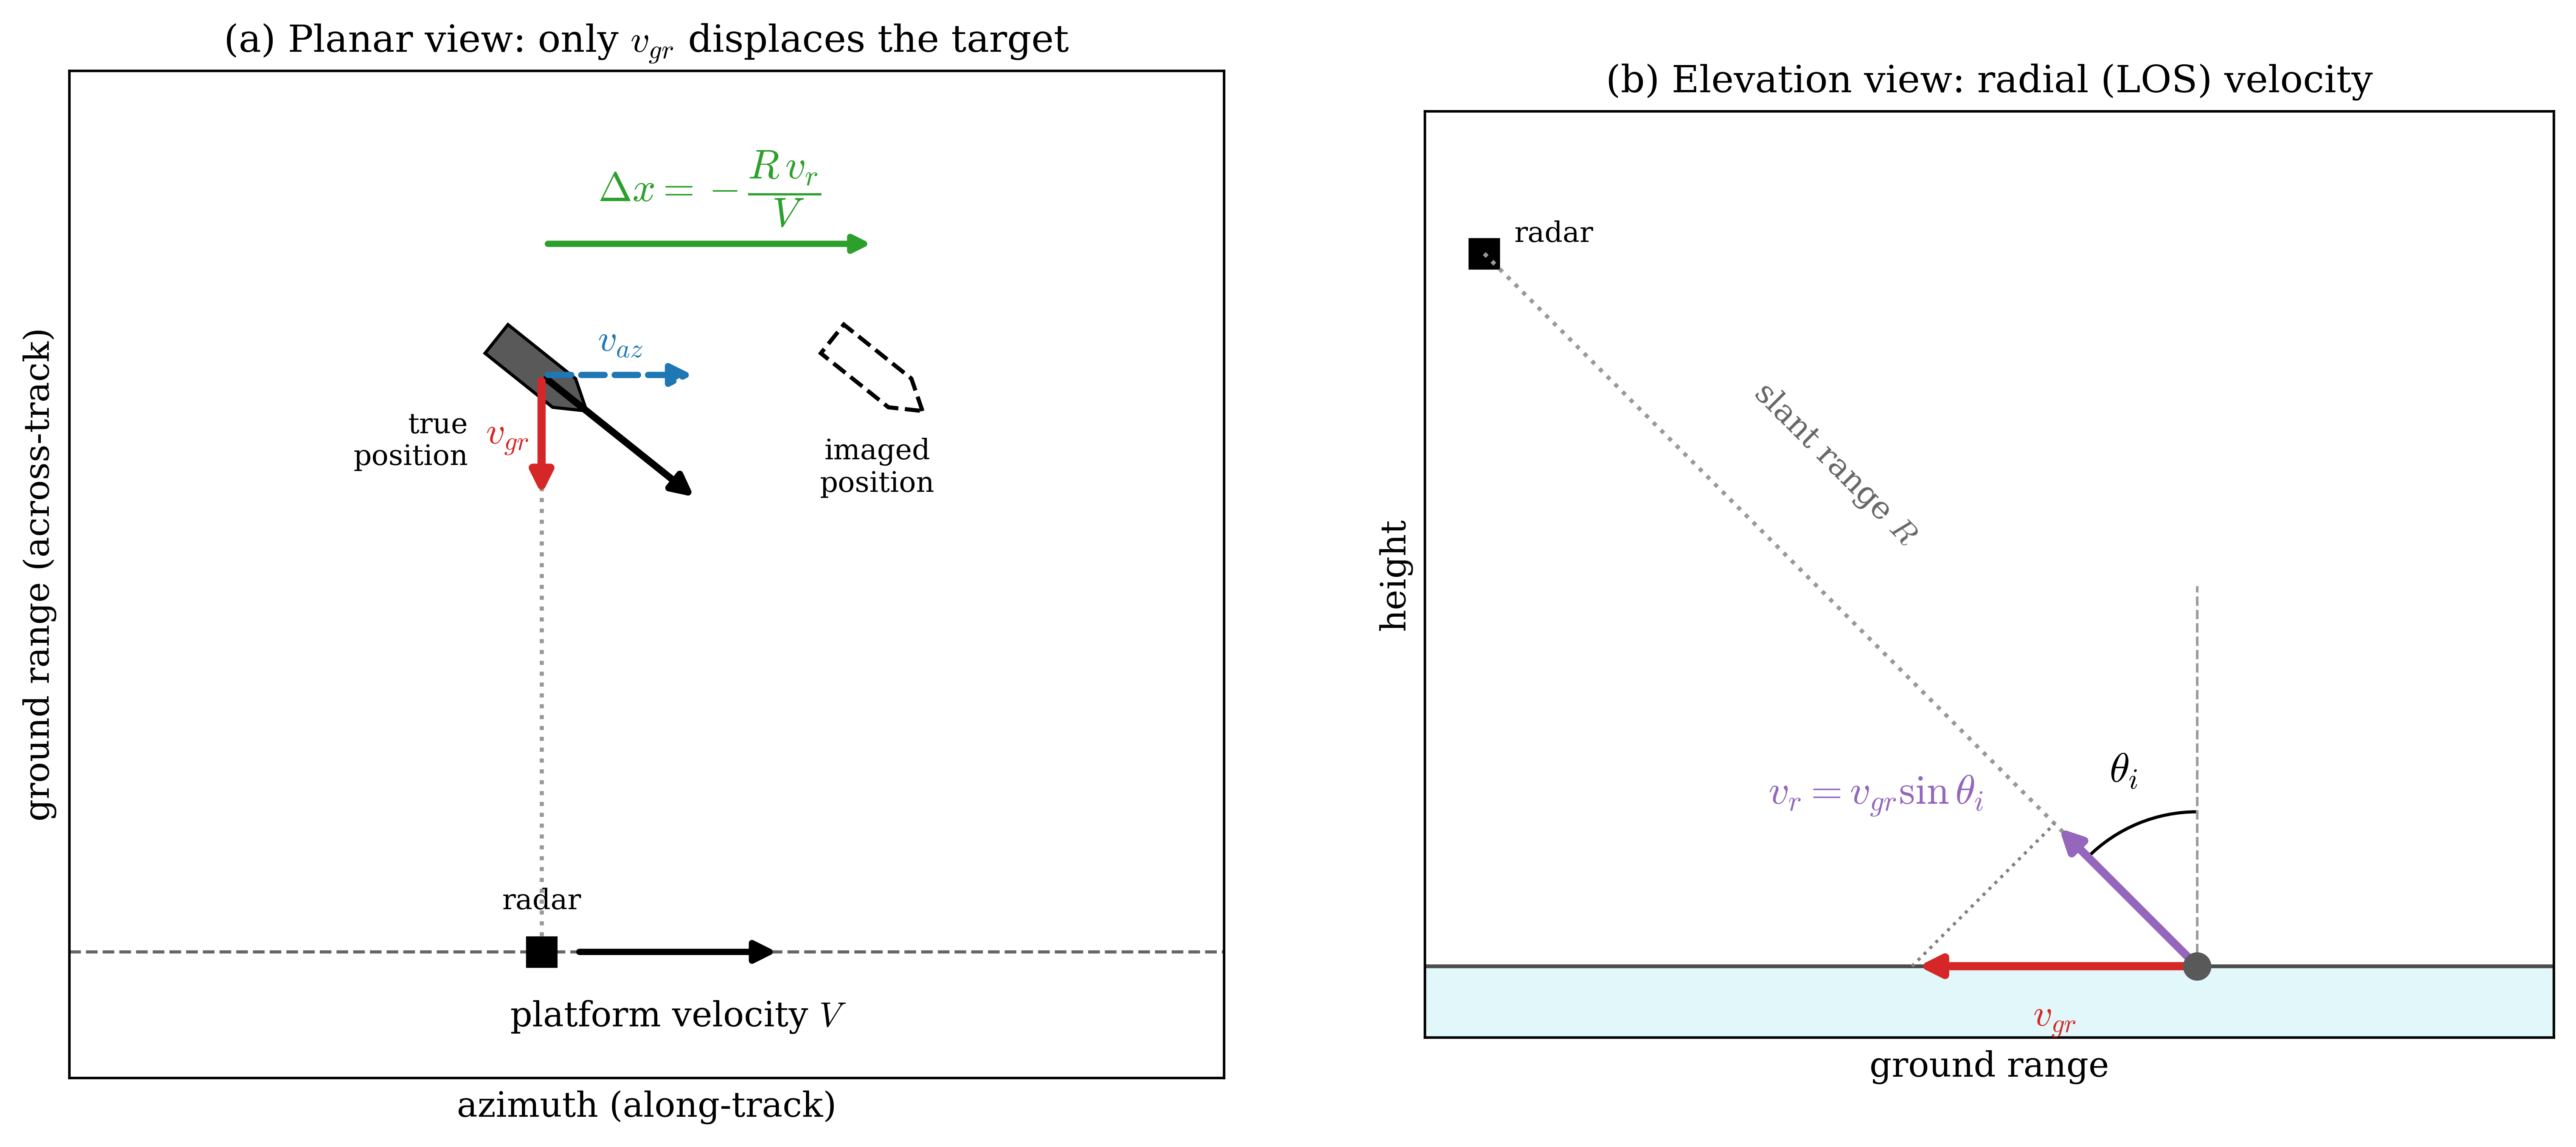
\includegraphics[width=0.95\textwidth]{Images/sar_azimuth_shift.png}
    \caption{Depicting the geometry of SAR azimuth shift. Subfigure $(a)$ shows the decomposed target velocity vector alongside the velocity vector of the radar platform. Subfigure $(b)$ shows the projected velocity component into the line of sight. This is the component that causes the Doppler offset.}
    \label{fig:sar_azimuth_shift}
\end{figure}

Since the azimuth shift is a known deterministic phenomenon, it can be compensated for. The main difficulty regarding compensation is that the velocity vector of the moving target must be known. This is fine for simulating measurements, but robust estimation of velocity in a multi target tracking scenario may be infeasible. It may also be unwanted, since using estimated states to compensate the measurement ruins the linear assumptions of the filtering, and may cause unforeseen consequences.
\medskip

There are two other ways one could incorporate azimuth shift in the measurement model. One alternative is to increase the noise of each measurement based on the absolute velocity of each vessel. It is generally easier to get a good estimate of how fast something is moving than to estimate the direction as well. This yields the measurement model below and may yield better results than estimating the exact azimuth shift. It does however also invalidate the linear assumptions of the filter and needs to be tested rigorously in various conditions.
\[
z = Hx + v(\nu), \quad H = \begin{bmatrix} I & 0 \end{bmatrix}
\]
With the noise $v(\nu)$ is defined as
\[
v(\nu) \sim \mathcal{N}(\mathbf{0}, \mathbf{R}(\nu))
\]
Where $\mathbf{R}$ is the measurement noise covariance matrix.
\medskip

The last approach is to just increase the measurement noise, but keep it constant for all measurements. This keeps the filter linear and is in many ways the ``safest'', but it will reduce the value of measurements where the vessel is at low velocity.
\medskip

It is also worth noting that SAR detectors could possibly return more information than just positions, but that will not be considered in this report.

\subsubsection{Navigation Radar Detector (NRD)}
NRD is a satellite borne detector, which tracks and locates the radar signals from civilian navigation radars \cite{nrd_ffi}. For tracking this means that the detector can be abstracted away, leaving a pure position measurement. What is special about NRD is that it can report the uncertainty of the measurement alongside each measurement. This means $R$ can be individual to each measurement. In general, the uncertainty increases radially around the center point of our measurement. This is useful for both simulation and filtering since the uncertainty is dependent on the measurement position and not the state position. One strength with NRD is that since it only detects radar signals, false positives are almost non-existent. This means that the measurements can be assumed to have a clutter intensity of almost zero. The measurement model, stated for completeness is then:

\[
z_i = Hx + v_i, \quad H = \begin{bmatrix} I & 0 \end{bmatrix}
\]
With the noise $v_i$ is defined as
\[
v_i \sim \mathcal{N}(\mathbf{0}, \mathbf{R}_i)
\]
Where $\mathbf{R}_i$ is the measurement noise covariance matrix, which is individual to each measurement.

\subsubsection{Electro-optical (EO) measurements}
As with both SAR and NRD, Electro-optical detectors are complicated and best abstracted away. Again, we are left with a direct position measurement on the form:

\[
z = Hx + v, \quad H = \begin{bmatrix} I & 0 \end{bmatrix}
\]
With the noise $v$ is defined as
\[
v \sim \mathcal{N}(\mathbf{0}, \mathbf{R})
\]
Where $\mathbf{R}$ is the measurement noise covariance matrix. In the case of EO, the variance is not reported by the sensor, thus we model all measurements with the same covariance matrix $\mathbf{R}$.